\documentclass[11pt,a4paper]{article}

% ---------------------------------------------------------------------------
% Packages (matched to the existing project reports)
% ---------------------------------------------------------------------------
\usepackage[T1]{fontenc}
\usepackage[utf8]{inputenc}
\usepackage[htt]{hyphenat}
\setlength{\emergencystretch}{3em}
\usepackage[a4paper,margin=2.4cm]{geometry}
\usepackage{graphicx}
\usepackage{subcaption}
\usepackage{booktabs}
\usepackage{longtable}
\usepackage{tabularx}
\usepackage{array}
\usepackage{enumitem}
\usepackage{caption}
\usepackage{float}
\usepackage{xcolor}
\usepackage[hidelinks]{hyperref}
\usepackage{url}

\graphicspath{{figures/}}
\captionsetup{font=small,labelfont=bf}
\setlist{topsep=2pt,itemsep=1pt,parsep=0pt}
\newcolumntype{L}[1]{>{\raggedright\arraybackslash}p{#1}}
\newcommand{\code}[1]{\texttt{#1}}

\title{\textbf{Agent Design Report}\\[0.4em]
\large A Governed Multi-Agent Architecture for Autonomous\\
E-Commerce and Accounting Operations}
\author{Research Engineer / System Architect\\\small Governed Multi-Agent AI for Autonomous E-Commerce and Accounting Operations}
\date{\today}

\begin{document}

% ===========================================================================
% TITLE PAGE
% ===========================================================================
\begin{titlepage}
\centering
\vspace*{1.4cm}
{\Huge\bfseries Agent Design Report\par}
\vspace{0.5cm}
{\Large A Governed Multi-Agent Architecture for Autonomous\\[2pt] E-Commerce and Accounting Operations\par}
\vspace{1.0cm}
{\large Design specification grounded in the inspected project repository\par}
\vspace{1.6cm}
\vfill
\begin{tabular}{rl}
\textbf{Document type:} & Agent design and implementation-status report \\[4pt]
\textbf{Architecture:} & Seven governed agents (Orchestrator, E-Commerce, \\
 & Inventory, Accounting, Risk/Anomaly, Governance, Audit) \\[4pt]
\textbf{Evidence base:} & \code{reports/dataset\_report/} (dataset analysis package), \\
 & \code{reports/dataset\_selection\_table/} (project/dataset overview), \\
 & \code{datasets/} (Olist CSV, Online Retail II XLSX) \\[4pt]
\textbf{Diagrams:} & \code{figures/} (generated by \code{figures/make\_figures.py}) \\[4pt]
\textbf{Date:} & \today \\
\end{tabular}
\vfill
{\small\itshape Integrity note. This report distinguishes, at every point, (i) components that are \emph{implemented} in the repository, (ii) components that are \emph{designed but not implemented}, and (iii) components that are \emph{proposed for future work}. Repository inspection found no agent implementation; consequently all seven agents are documented as proposed. This is stated explicitly rather than implied.}
\end{titlepage}

% ===========================================================================
% ABSTRACT
% ===========================================================================
\begin{abstract}
\noindent
This report specifies a seven-agent, governance-first architecture for the research project \emph{Governed Multi-Agent AI for Autonomous E-Commerce and Accounting Operations}, and documents its implementation status strictly from evidence found in the project repository. The seven agents are an Orchestrator/Coordination agent, an E-Commerce Operations agent, an Inventory Management agent, an Accounting agent, a Risk/Anomaly-Detection agent, a Governance/Policy-Enforcement agent, and an Audit/Traceability agent. Repository inspection established that \textbf{no agent code, message bus, policy engine, or audit ledger is present}: the only implemented software is (i) a reproducible dataset-analysis and validation package under \code{reports/dataset\_report/analysis/} --- which corresponds to the project's prospective \emph{ingestion and validation} layer and which produced the measured facts reused in this report --- and (ii) a standard-library dataset inspector under \code{reports/dataset\_selection\_table/scripts/}. All seven agents are therefore \emph{proposed}: they have a specified purpose, inputs, outputs, internal workflow, dependencies, governance requirements, failure handling and evaluation plan, but no executable realisation. The architecture operates over two independent, read-only datasets (the Olist Brazilian E-Commerce dataset and Online Retail II), ingested through separate source adapters that must never be record-level merged. Governance is modelled as an explicit lifecycle (request $\rightarrow$ planning $\rightarrow$ authorization $\rightarrow$ execution $\rightarrow$ validation $\rightarrow$ risk assessment $\rightarrow$ human approval $\rightarrow$ audit $\rightarrow$ response), and the report states which controls would be enforced in code and which currently remain design recommendations. Evaluation is presented as a \emph{proposed} protocol because no agent experiments have yet been run. Every numerical dataset fact cited here is measured by the accompanying analysis package and reported in the project's \emph{Dataset Report}; no implementation, test result, performance figure, or capability is fabricated.
\end{abstract}

\tableofcontents
\clearpage

% ===========================================================================
% GLOSSARY
% ===========================================================================
\section*{Glossary of Abbreviations}
\addcontentsline{toc}{section}{Glossary of Abbreviations}
\begin{tabularx}{\textwidth}{L{2.6cm}X}
\toprule
\textbf{Term} & \textbf{Meaning} \\ \midrule
Agent & A software component with an explicit role, inputs, outputs and a governance-wrapped interface. \\
Audit event & A prototype-generated, append-only record of an agent action and its decision context. \\
BRL & Brazilian Real, the currency implied by the Olist marketplace context. \\
Canonical event & A minimal, source-tagged internal representation shared across adapters where a defensible mapping exists. \\
Evidence reference & A pointer to the source record(s) (table + key) that justify a decision. \\
FK & Foreign key. \\
GBP (\pounds) & Pound sterling, the currency of Online Retail II. \\
Governance & The set of explicit policies and checks that constrain agent actions (allow / block / escalate). \\
Human-in-the-loop & A required human approval step for high-impact actions defined by policy. \\
Orchestrator & The agent that plans tasks, delegates to specialists and consolidates results. \\
PK & Primary key. \\
Proposed & Designed in this report but not implemented in the repository. \\
Implemented & Present as executable code in the repository (evidenced by file and function references). \\
Source adapter & Read-only component that ingests one dataset and emits canonical events. \\
\bottomrule
\end{tabularx}

% ===========================================================================
\section{Executive Summary}
% ===========================================================================
The project investigates how a set of specialised, governed software agents can cooperate to perform e-commerce and accounting-related workflows while remaining traceable and auditable. This report turns the project's conceptual agent roles into a concrete design specification, and --- critically --- separates that specification from the current state of the repository.

\paragraph{What was found.} A full inspection of the repository (see Appendix~\ref{app:inventory}) identified exactly three substantive content areas: the raw datasets under \code{datasets/}; a dataset-analysis report and package under \code{reports/dataset\_report/}; and a dataset-selection report and inspector under \code{reports/dataset\_selection\_table/}. There is \textbf{no agent code} anywhere in the repository: no orchestrator, no message schemas, no policy engine, no audit store, and no test that exercises agent behaviour. The directory \code{src/} is empty and the root \code{README.md} is empty. Accordingly, \textbf{every one of the seven agents is classified as \emph{proposed}} in this report.

\paragraph{What is implemented.} The only executable software relevant to the project is the dataset-analysis package (\code{reports/dataset\_report/analysis/}), which reads the raw files read-only and computes schema validation, candidate-key checks, referential-integrity checks, join-inflation measurement, missingness and duplicate profiling, temporal and monetary summaries, a payment-versus-item reconciliation proxy, business-signal detection, and figures. This package is, in effect, a working prototype of the project's \emph{ingestion and validation} layer and is the foundation on which the agents would be built. A second, independent inspector (\code{reports/dataset\_selection\_table/scripts/inspect\_datasets.py}) performs a standard-library inventory and quality scan. The analysis package is covered by thirteen unit tests, all of which were executed and pass; these tests, however, validate data metrics, not agent behaviour.

\paragraph{Datasets.} Two independent datasets supply evidence: Olist (nine relational CSVs; 1{,}550{,}922 rows) as the primary source for multi-table e-commerce workflows, and Online Retail II (two worksheets; 1{,}067{,}371 invoice lines) as a complementary transaction-level source. Neither contains inventory stock levels, a general ledger, explicit governance policies, or verified fraud labels. These limitations are inherited by the agent design and are stated throughout.

\paragraph{Governance and audit.} Governance is specified as an explicit, versioned lifecycle applied to every agent action, with a separation between \emph{recommendation} and \emph{execution}, and with human approval required for policy-defined high-impact actions. Because none of this is implemented, all such controls are presented as design recommendations, and the report is explicit about the resulting gap between design and enforcement.

% ===========================================================================
\section{Introduction and Research Motivation}
% ===========================================================================
\subsection{Motivation}
Business operations such as order fulfilment and accounting reconciliation are inherently \emph{multi-step} and \emph{cross-functional}: a purchase triggers payment capture, fulfilment, invoicing and, later, reconciliation and reporting. Each step has different data, different failure modes and different control requirements. This structure motivates a division of labour among specialised agents \cite{wooldridge2009,shoham2009}, each an expert over a narrow slice of the workflow.

\subsection{Why a single unrestricted agent is insufficient}
A single agent with broad permissions faces three problems that motivate the governance-first design:
\begin{enumerate}
\item \textbf{Separation of duties.} Accounting and audit controls rely on the principle that the same actor should not both propose and approve a consequential action \cite{coso2013,sox2002}. A monolithic agent collapses these roles.
\item \textbf{Focused validation.} Different tasks require different validations (schema and key integrity for ingestion; amount reconciliation for accounting; distributional and temporal checks for anomaly detection). Specialised agents allow each validation to be explicit and testable.
\item \textbf{Traceability.} When one component does everything, it is hard to isolate which step produced a given outcome. An orchestrated set of agents with an audit trail yields finer-grained traceability, which is a prerequisite for trustworthy automation \cite{nistAirmf2023}.
\end{enumerate}

\subsection{Scope of this report}
The report specifies the seven-agent architecture, its interfaces, its governance model, its mapping onto the two datasets, four end-to-end scenarios, proposed data contracts, a proposed evaluation protocol, failure modes, and an implementation roadmap. Throughout, it preserves the terminology and dataset findings already established in the project's \emph{Dataset Report} (Deliverable~2, the dataset analysis) and \emph{project overview} (Deliverable~1, the dataset-selection report), and it does not re-derive the dataset analysis.

% ===========================================================================
\section{System Objectives and Scope}
% ===========================================================================
\subsection{Objectives}
\begin{itemize}
\item \textbf{O1.} Provide a coordination layer that decomposes a user request into tasks and routes them to specialised agents.
\item \textbf{O2.} Ground each specialised agent in the two available datasets through read-only adapters, without fabricating data that the sources do not contain.
\item \textbf{O3.} Enforce explicit, versioned governance policies on every agent action, with human approval for high-impact actions.
\item \textbf{O4.} Produce an append-only audit trail that links each recommendation to the evidence that justified it.
\item \textbf{O5.} Support a reproducible evaluation of coordination, validation, reconciliation and governance behaviour.
\end{itemize}

\subsection{Expected users}
The primary users are the research team and a supervisor evaluating the prototype; secondary (future) users are operations and finance staff in a hypothetical adopter. No end-user interface exists at present.

\subsection{Operational scope and assumptions}
\begin{itemize}
\item The system operates in \textbf{offline replay mode} over historical datasets; it does not connect to live commerce or accounting systems.
\item The two datasets are treated as \textbf{independent evidence sources}. They differ in currency (BRL vs.\ \pounds), period, schema and semantics, and \textbf{must not be record-level merged}.
\item Monetary and temporal analyses are \textbf{analytical}: they are not ledger postings or audited statements.
\item Anomalies are \textbf{candidate} signals, not fraud determinations.
\end{itemize}

\subsection{Prototype versus production}
This is a \textbf{research prototype}. It is not a production-ready autonomous business platform: it lacks persistent operations, authentication, real tools, transactional settlement, and any operational deployment. The distinction is maintained deliberately, so that no reader infers production capability from the design.

% ===========================================================================
\section{Overall System Architecture}
% ===========================================================================
\subsection{Overview}
The architecture comprises seven agents organised in layers: a coordination layer (Orchestrator); four operational/analytical layers (E-Commerce, Inventory, Accounting, Risk); a governance layer that gates every action; and an audit layer that records every action. Data reach the agents only through read-only source adapters. Figure~\ref{fig:arch} shows the proposed structure, with \textbf{solid borders for the one implemented component} (the ingestion and validation layer) and \textbf{dashed borders for all proposed components}.

\begin{figure}[H]\centering
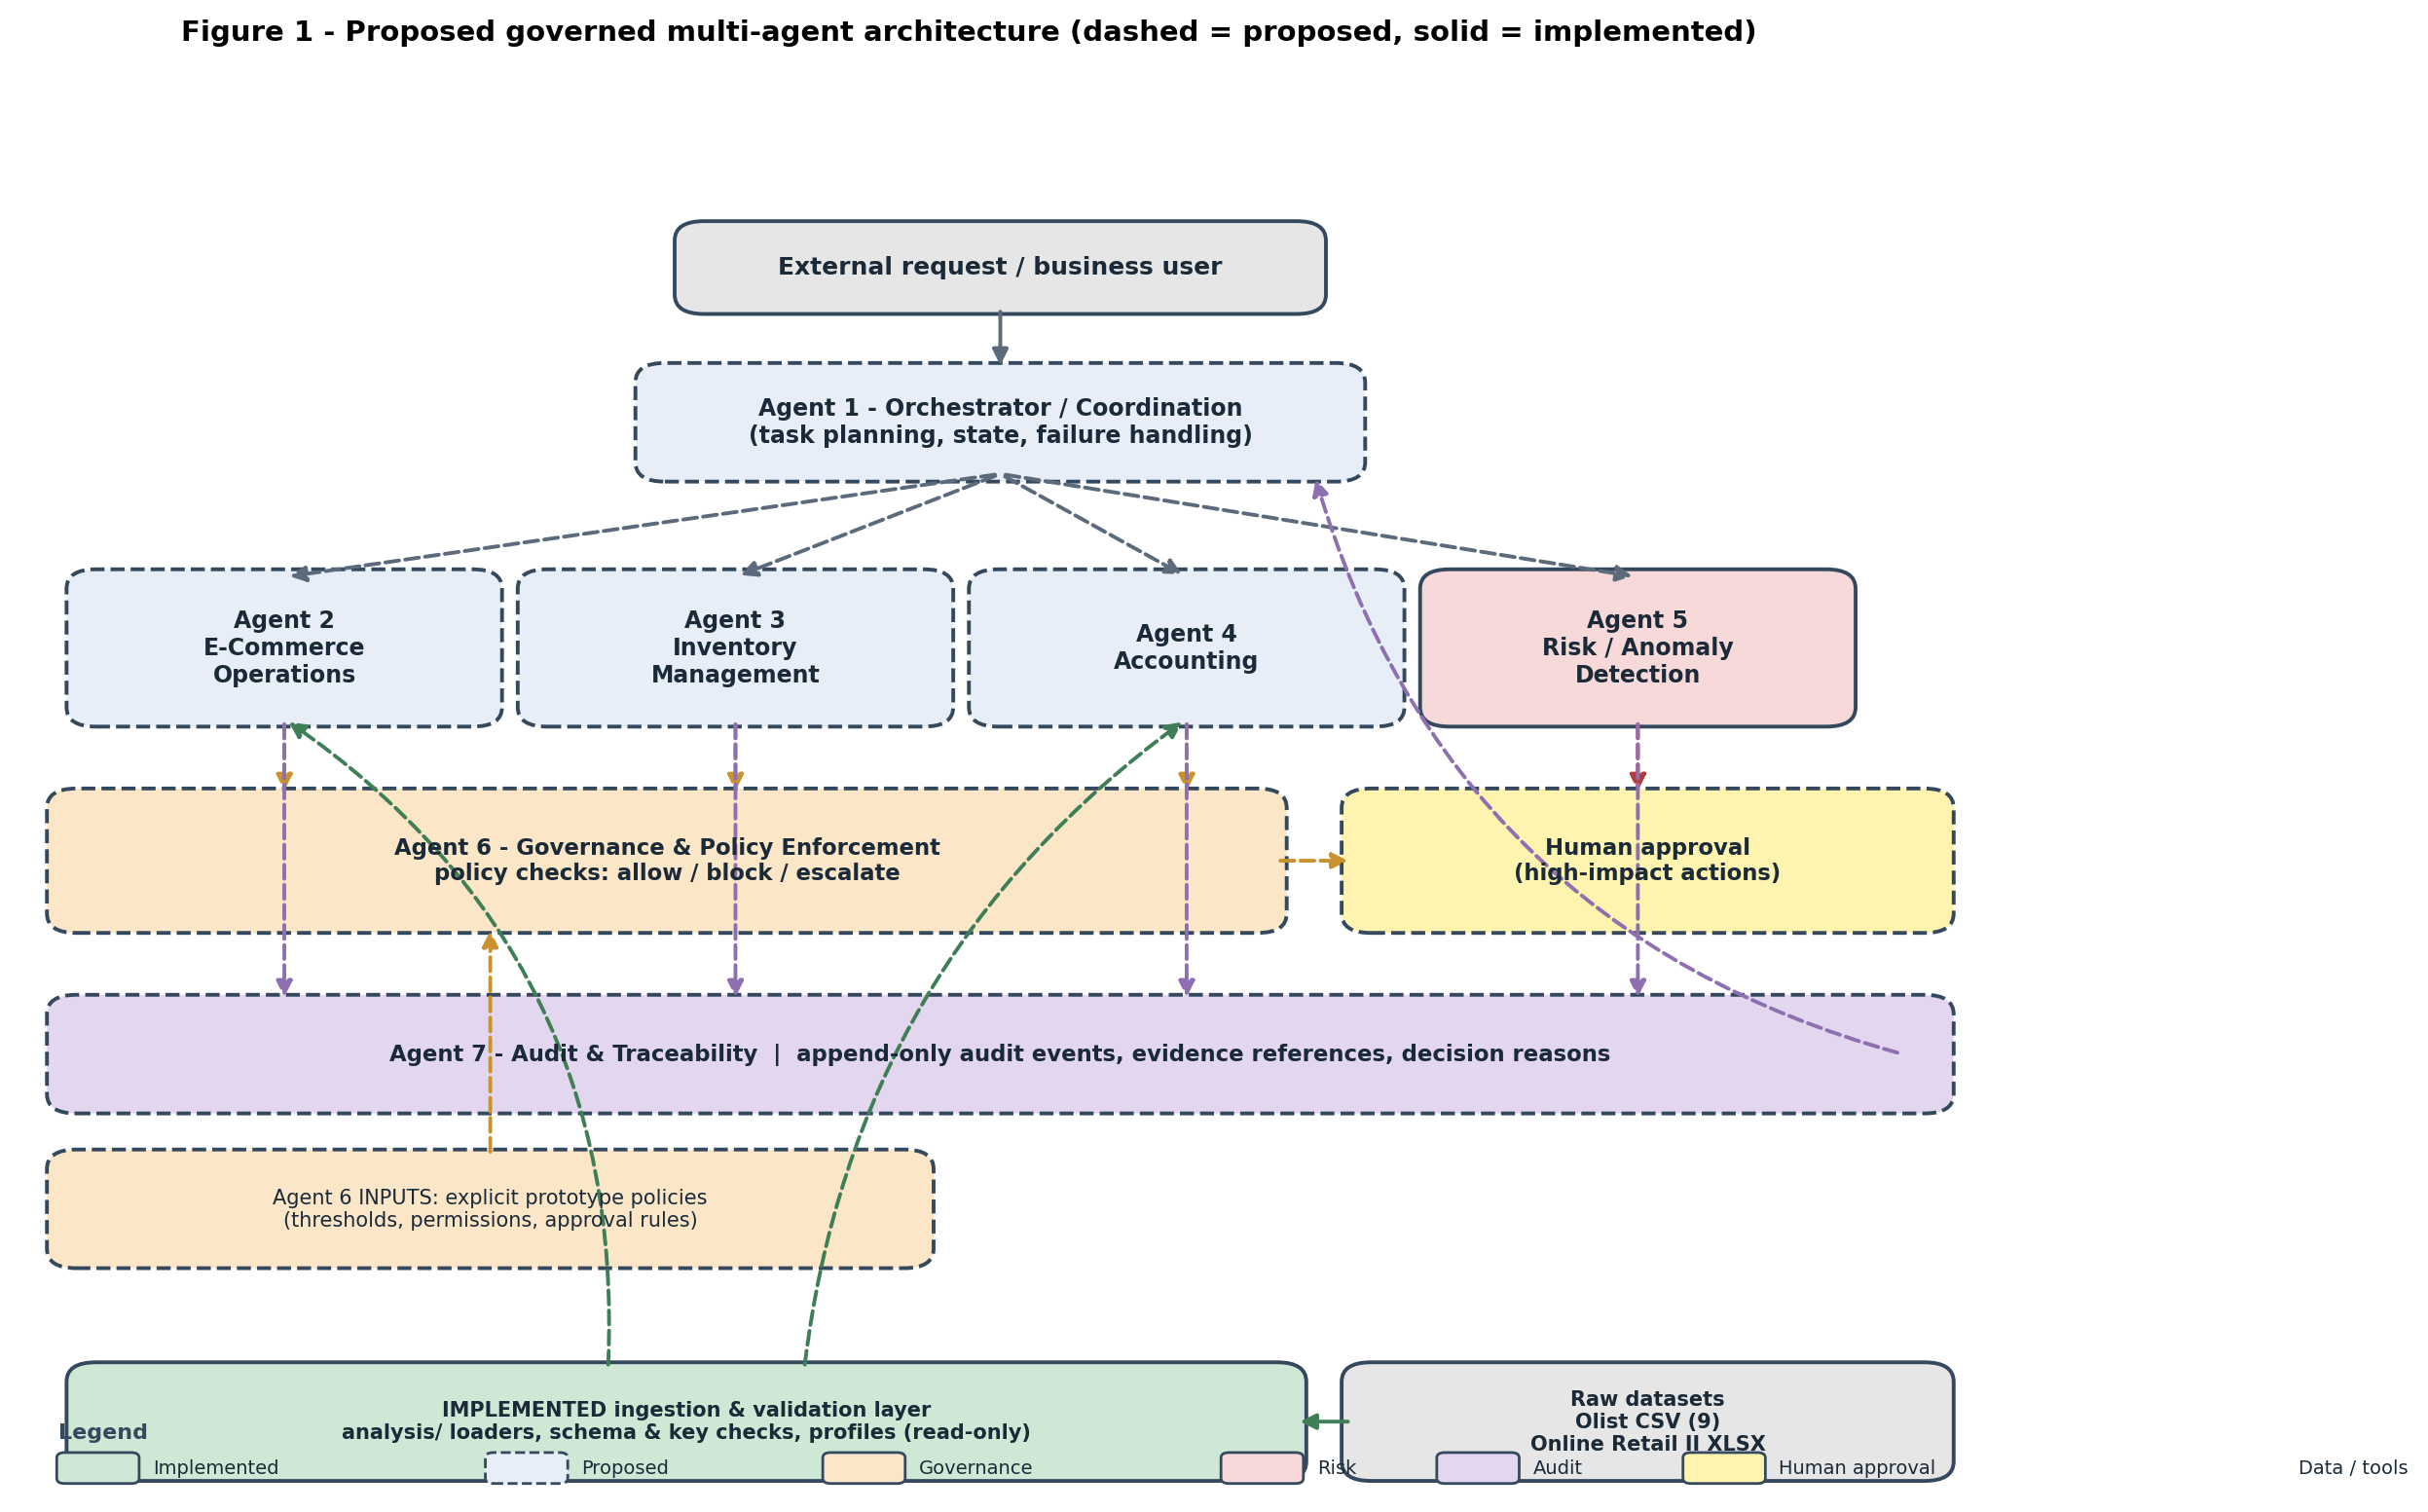
\includegraphics[width=\textwidth]{fig_architecture.png}
\caption{Proposed governed multi-agent architecture. Dashed components are proposed and not implemented; the solid component is the implemented dataset ingestion and validation layer.}
\label{fig:arch}
\end{figure}

\subsection{Implementation status of the architecture}
Figure~\ref{fig:status} summarises the status observed during repository inspection. It separates the seven proposed agents from the two implemented data-layer components. No arrow, message, policy rule or audit record in the architecture is currently realised in code.

\begin{figure}[H]\centering
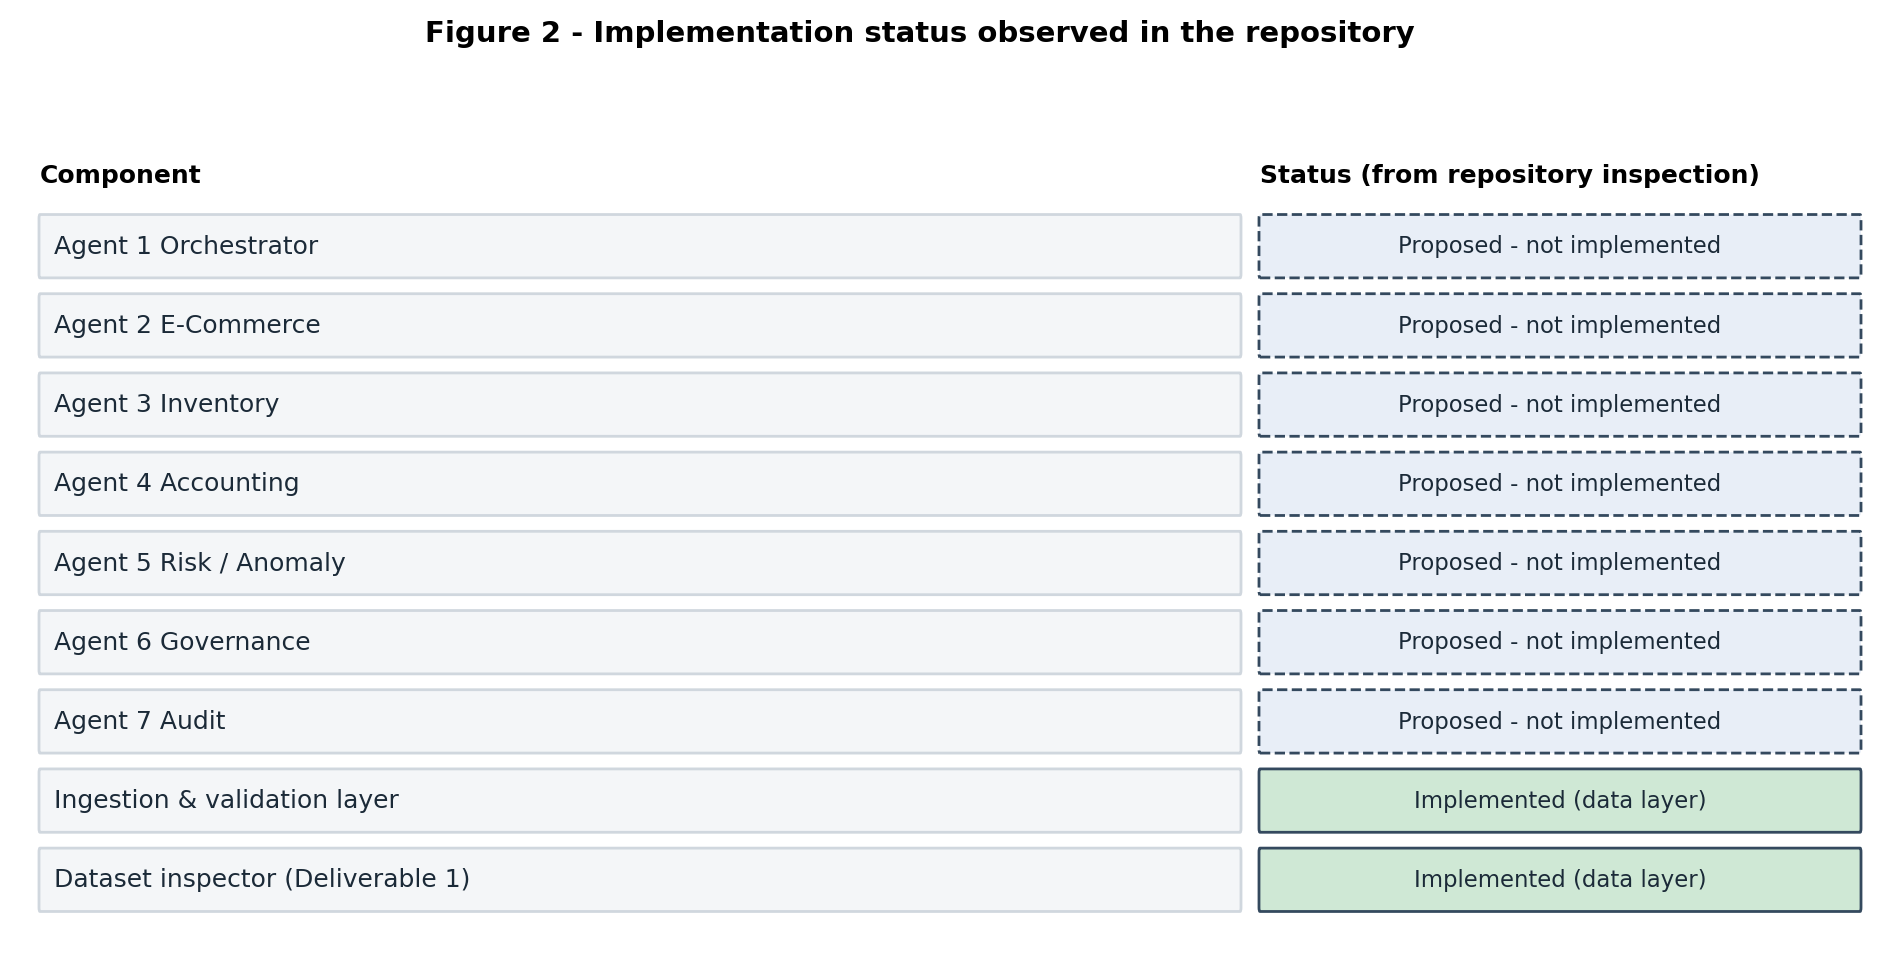
\includegraphics[width=\textwidth]{fig_status_matrix.png}
\caption{Implementation status per architectural component, observed directly from the repository. The data layer is implemented; all agents are proposed.}
\label{fig:status}
\end{figure}

\subsection{Interaction summary}
At a high level, a request enters the Orchestrator (Agent~1). The Orchestrator plans tasks and invokes the relevant operational agents (Agents~2--5). Each operational agent reads canonical events derived by the source adapters, produces a structured result, and submits any consequential action to the Governance agent (Agent~6). The Governance agent returns allow/block/escalate, optionally requiring human approval. Every action and decision is handed to the Audit agent (Agent~7). The Orchestrator then consolidates a recommendation for the user. The governance and audit interactions are described in Sections~\ref{sec:comms} and~\ref{sec:governance}.

% ===========================================================================
\section{Individual Agent Specifications}
% ===========================================================================
\label{sec:agents}
This section specifies each agent using a common structure: purpose; inputs; outputs; internal workflow; tools and data sources; interactions; governance requirements; error handling; implementation status; and limitations. The implementation status is repeated verbatim from inspection: \textbf{all seven agents are proposed / not implemented}. Where an agent could reuse the implemented analysis package, this is noted explicitly.

% ---------------------------------------------------------------------------
\subsection{Agent 1 --- Orchestrator / Coordination Agent}
\paragraph{Purpose and responsibilities.} Receive a user request, translate it into structured tasks, determine which specialised agents are required, sequence their execution, maintain workflow state, detect failures/timeouts/conflicts, ensure governance checks are invoked, and return a consolidated, traceable result.

\paragraph{Inputs (schema).} \code{UserRequest} (see Section~\ref{sec:contracts}): a natural-language or structured goal, requester identity, and an optional scope (dataset, entity, time window).

\paragraph{Outputs (schema).} \code{WorkflowResult}: the consolidated recommendation, the ordered task list with per-task status, the set of agent results, the governance decisions, and the audit event identifiers that reference the supporting evidence.

\paragraph{Internal workflow.} (i) Parse and validate the request; (ii) decompose into a directed acyclic task graph; (iii) resolve data scope through the source adapters; (iv) invoke agents in dependency order; (v) route consequential actions through governance; (vi) on success, consolidate; on failure, apply the fallback policy (retry, degrade, or escalate); (vii) record the workflow to the audit trail.

\paragraph{Tools, APIs, libraries, data sources.} No orchestration framework is present. The Orchestrator would be implemented over the implemented analysis layer for data access and a to-be-built task/message runtime. Candidate libraries would be chosen by the implementer; none is currently in the repository.

\paragraph{Interactions.} Calls Agents~2--5; consults Agent~6 before any consequential action; writes to Agent~7; returns results to the user.

\paragraph{Governance and validation.} Must not execute consequential actions directly; must route them through Agent~6; must attach evidence references to every recommendation.

\paragraph{Error handling and fallback.} Detects agent failure, timeout, and contradictory outputs; degrades gracefully by returning partial results clearly marked as incomplete; escalates to a human when policy requires.

\paragraph{Implementation status.} \textbf{Proposed.} No orchestration code exists. Related implemented capability: none (data access only, via the analysis package).

\paragraph{Limitations and future improvements.} Coordination behaviour cannot be validated from historical data; it must be exercised by the prototype and evaluated through its own traces. Circular delegation must be prevented by construction (a task graph with a depth limit).

% ---------------------------------------------------------------------------
\subsection{Agent 2 --- E-Commerce Operations Agent}
\paragraph{Purpose and responsibilities.} Analyse orders, customers, products, sellers, payments and reviews; support order-related workflows; identify incomplete or inconsistent order information; provide structured operational recommendations; coordinate with the Inventory, Accounting, Risk and Governance agents.

\paragraph{Inputs (schema).} Canonical order/transaction events and line items derived from Olist (orders joined to items, payments, reviews) and from Online Retail II (invoice lines). Relevant Olist fields include \code{order\_id}, \code{order\_status}, the order timestamps, \code{payment\_type}, \code{payment\_value} and \code{review\_score}; Online Retail II fields include \code{Invoice}, \code{StockCode}, \code{Quantity}, \code{InvoiceDate} and \code{Country}.

\paragraph{Outputs (schema).} \code{OperationsSummary} and \code{OperationsRecommendation}: order/transaction volumes, status distributions, sales aggregates, cancellation analysis, and flagged completeness/inconsistency issues, each with evidence references.

\paragraph{Internal workflow.} Retrieve scoped records; compute aggregates (status distribution, monthly volume, category revenue, cancellation rate); apply completeness checks (e.g.\ orders lacking items/payment/review); emit structured findings.

\paragraph{Tools, APIs, libraries, data sources.} The implemented analysis package already computes the underlying aggregates: Olist status/payment/review value counts, monthly order volumes and category revenue (\code{analysis/olist.py}; \code{analysis/figures.py}), and Online Retail II monthly activity and cancellation metrics (\code{analysis/online\_retail.py}). No live e-commerce access exists.

\paragraph{Interactions.} Receives tasks from Agent~1; shares demand signals with Agent~3; shares transaction amounts with Agent~4; shares completeness/inconsistency signals with Agent~5; submits recommendations to Agent~6; logs to Agent~7.

\paragraph{Governance and validation.} Read-only analysis may proceed under authorization; any recommendation that would change a record must go through Agent~6.

\paragraph{Error handling and fallback.} Returns explicit ``not available in source dataset'' markers rather than imputing missing fields; aborts a task if a required schema is missing (mirroring the implemented schema checks).

\paragraph{Implementation status.} \textbf{Proposed as an agent.} The analytical computations it would expose are \emph{partially implemented} as library functions in the analysis package, but there is no agent wrapper, interface, or workflow.

\paragraph{Limitations and future improvements.} Olist has no marketing/session/acquisition data; Online Retail II has no order-status concept and 22.77\% of lines lack a customer identifier, limiting customer-centric analysis.

% ---------------------------------------------------------------------------
\subsection{Agent 3 --- Inventory Management Agent}
\paragraph{Purpose and responsibilities.} Analyse product and order-item data to characterise demand; identify possible stock-related risks and availability concerns; produce demand indicators and inventory recommendations \emph{where the data supports them}; communicate findings to the Orchestrator and E-Commerce agent.

\paragraph{Inputs (schema).} Olist order items (\code{product\_id}, \code{order\_item\_id}, \code{price}, \code{freight\_value}, \code{shipping\_limit\_date}) and product attributes; Online Retail II lines (\code{StockCode}, \code{Quantity}, \code{InvoiceDate}). No stock-on-hand field exists in either source.

\paragraph{Outputs (schema).} \code{DemandIndicator} per product (units sold, demand variability) and a \emph{qualified} \code{InventoryRecommendation} that explicitly states it is a demand proxy, not a replenishment decision.

\paragraph{Internal workflow.} Aggregate units sold per product; compute variability and a days-without-sales proxy; rank products; attach an explicit ``no stock data'' limitation to every recommendation.

\paragraph{Tools, APIs, libraries, data sources.} The implemented package computes per-product category revenue and value counts (\code{analysis/olist.py}); quantity/price distributions and monthly activity for Online Retail II (\code{analysis/online\_retail.py}).

\paragraph{Interactions.} Consumes canonical lines; receives demand context from Agent~2; flags data gaps to Agent~6; logs to Agent~7.

\paragraph{Governance and validation.} Must not present demand proxies as actual stock positions; any downstream action requires policy validation.

\paragraph{Error handling and fallback.} If product attributes are missing (610 products lack category metadata in Olist; 1.85\%), it degrades to line-level quantity analysis and marks the gap.

\paragraph{Implementation status.} \textbf{Proposed.} Only the underlying demand aggregations exist; no inventory logic, stock model, or replenishment reasoning is implemented.

\paragraph{Limitations and future improvements.} \textbf{Neither dataset contains stock quantities, warehouse records, replenishment history, or inventory snapshots.} Inventory management is therefore an \emph{analytical prototype only}; real stock decisions would require an external inventory source. Listed as a hard limitation throughout.

% ---------------------------------------------------------------------------
\subsection{Agent 4 --- Accounting Agent}
\paragraph{Purpose and responsibilities.} Analyse payment records, order values and transaction totals; reconcile related records where the fields permit; identify discrepancies requiring investigation; produce structured accounting summaries; send suspicious discrepancies to the Risk agent and relevant decisions to the Governance agent.

\paragraph{Inputs (schema).} Olist \code{order\_payments} (\code{payment\_value}, \code{payment\_type}, \code{payment\_installments}) and \code{order\_items} (\code{price}, \code{freight\_value}); Online Retail II line value (\code{Quantity} $\times$ \code{Price}), cancellations and adjustments.

\paragraph{Outputs (schema).} \code{ReconciliationResult} (order identifier, item total, payment total, absolute difference, match flag) and \code{AccountingSummary} (aggregate totals clearly labelled as analytical, not ledger postings).

\paragraph{Internal workflow.} Sum item value (price + freight) per order; sum payment value per order; join on \code{order\_id}; compute differences; flag mismatches beyond a threshold; forward flagged cases.

\paragraph{Tools, APIs, libraries, data sources.} The implemented package already computes an order-level reconciliation proxy: of the 98{,}665 orders with both items and payments, 98{,}287 (99.62\%) agree within one cent, mean absolute difference 0.0332 BRL (\code{analysis/olist.py}, \code{facts["reconciliation\_proxy"]}). It also computes monetary totals (item prices 13{,}591{,}643.70 BRL; freight 2{,}251{,}909.54 BRL; payments 16{,}008{,}872.12 BRL).

\paragraph{Interactions.} Receives tasks from Agent~1; receives transaction amounts from Agent~2; forwards discrepancies to Agent~5; submits decisions to Agent~6; logs to Agent~7.

\paragraph{Governance and validation.} Any adjustment or posting is a high-impact action requiring evidence and, per policy, human approval; the agent must never present an analytical total as a ledger entry.

\paragraph{Error handling and fallback.} If orders lack either items or payments, it reports the relationship gap (Olist: 775 orders without items, 1 without payment) rather than forcing a reconciliation.

\paragraph{Implementation status.} \textbf{Proposed as an agent.} The \emph{reconciliation proxy} is implemented as a data computation; there is no accounting agent, no journal, and no ledger.

\paragraph{Limitations and future improvements.} No general ledger, chart of accounts, tax records, settlement statements, or audited statements exist in either dataset; the Olist reconciliation is an item-versus-payment proxy only.

% ---------------------------------------------------------------------------
\subsection{Agent 5 --- Risk and Anomaly Detection Agent}
\paragraph{Purpose and responsibilities.} Identify unusual transactions, inconsistencies and suspicious patterns; examine cancellations, negative quantities/values, unusual payment patterns and data-quality issues; produce structured anomaly signals with explanations and confidence information where supported; prioritise cases for review; share findings with the Accounting and Governance agents.

\paragraph{Inputs (schema).} Olist delivery-timing fields, monetary fields and review scores; Online Retail II \code{Quantity}, \code{Price}, invoice-prefix (cancellation) and missing-identifier fields.

\paragraph{Outputs (schema).} \code{AnomalySignal}: entity reference, rule/method, score, explanation, evidence reference, and an explicit category (data-quality error / operational anomaly / statistical outlier / potential financial risk). \textbf{Not} ``confirmed fraud''.

\paragraph{Internal workflow.} Apply transparent rules (e.g.\ delivered-before-carrier; negative quantity on non-cancellation invoices; zero/negative price; extreme quantity) and statistical fences (IQR) to flag candidates; attach explanations; rank by severity.

\paragraph{Tools, APIs, libraries, data sources.} The implemented package computes the relevant inputs: numeric statistics with IQR fences and sign counts (\code{analysis/profiling.py}), Online Retail II quality metrics (negative/zero/negative-price counts, cancellation rows) (\code{analysis/online\_retail.py}), and a temporal-integrity check that found 23 Olist orders recorded as delivered to the customer before carrier handoff (\code{analysis/olist.py}).

\paragraph{Interactions.} Receives tasks from Agent~1; receives discrepancies from Agent~4; escalates to Agent~6; logs to Agent~7.

\paragraph{Governance and validation.} Must label outputs as candidate anomalies; must not assert fraud; escalation is mandatory when evidence is insufficient.

\paragraph{Error handling and fallback.} If the required distribution is unavailable, it falls back to rule-based flags and states reduced confidence.

\paragraph{Implementation status.} \textbf{Proposed as an agent.} Rule inputs are implemented; no anomaly engine, scoring, or prioritisation exists.

\paragraph{Limitations and future improvements.} \textbf{No verified fraud labels exist}, so precision/recall cannot be computed from these data; the agent produces candidate signals only. Terminology follows the standard anomaly-detection survey \cite{chandola2009} and fraud-detection literature \cite{ngai2011}.

% ---------------------------------------------------------------------------
\subsection{Agent 6 --- Governance and Policy Enforcement Agent}
\paragraph{Purpose and responsibilities.} Validate every agent request against explicit policies; check authorization, permitted actions, required evidence and approval conditions; enforce human approval for high-impact actions; prevent unauthorized or unsupported actions; record policy decisions and reasons.

\paragraph{Inputs (schema).} \code{ActionRequest}: acting agent, action type, target, justification, and evidence references. Plus the active \code{PolicySet} (versioned).

\paragraph{Outputs (schema).} \code{PolicyDecision}: \code{allow} / \code{block} / \code{escalate}, the evaluated policy identifier, a reason, and (if required) a human-approval request.

\paragraph{Internal workflow.} Evaluate the action against the applicable policies; verify evidence sufficiency; determine impact level; return a decision; if high-impact and policy says so, raise a human-approval request.

\paragraph{Tools, APIs, libraries, data sources.} \textbf{No policy engine is implemented.} The dataset contains no policies, permissions or approval workflows; the policy set would be external configuration created by the prototype.

\paragraph{Interactions.} Called by every other agent before any consequential action; interacts with Agent~7 to record decisions and with the human approver.

\paragraph{Governance and validation.} This \emph{is} the governance control; it must be invoked on every action and must not be bypassable by operational agents.

\paragraph{Error handling and fallback.} Fail-closed: missing or contradictory evidence triggers escalation, never silent execution.

\paragraph{Implementation status.} \textbf{Proposed} (design only). Candidate policy rules are listed in Section~\ref{sec:governance}.

\paragraph{Limitations and future improvements.} Because governance is conceptual, this report labels all controls as proposed; implementing and testing them is the central future milestone.

% ---------------------------------------------------------------------------
\subsection{Agent 7 --- Audit and Traceability Agent}
\paragraph{Purpose and responsibilities.} Record workflow events, agent decisions, tool calls, validation outcomes and policy checks; maintain links between requests, intermediate results, anomalies and final recommendations; support investigation and reproducibility; capture timestamps, identifiers, reasons and evidence references.

\paragraph{Inputs (schema).} \code{AuditEvent}s emitted by all agents (see Section~\ref{sec:contracts}).

\paragraph{Outputs (schema).} An append-only event stream and reconstruction queries (``what evidence justified this recommendation?'').

\paragraph{Internal workflow.} Append each event with a unique identifier, timestamp and evidence references; never mutate or delete; support deterministic replay.

\paragraph{Tools, APIs, libraries, data sources.} \textbf{No audit store is implemented.} There is no append-only ledger, no cryptographic integrity check, and no tamper-proof storage. The analysis package does record input file hashes via \code{config.sha256\_file} and writes run artifacts, which is a limited precedent for reproducibility but not an audit ledger.

\paragraph{Interactions.} Receives events from all agents; provides traces to the Orchestrator and to a human investigator.

\paragraph{Governance and validation.} Must record every policy decision and its reason; must not store personal data (see privacy note in Section~\ref{sec:limitations}).

\paragraph{Error handling and fallback.} Detects missing audit fields and flags incomplete traces; if the store is unavailable, the workflow must fail closed rather than proceed unlogged.

\paragraph{Implementation status.} \textbf{Proposed.} Not implemented; the report does \emph{not} describe the audit system as immutable or tamper-proof.

\paragraph{Limitations and future improvements.} Audit records are prototype-generated and are not attributes of either dataset.

% ---------------------------------------------------------------------------
\subsection{Agent comparison}
Table~\ref{tab:agentsum} summarises the seven agents. The ``Base data'' column names the dataset evidence each agent would use; the ``Status'' column is fixed by repository inspection.

\begin{table}[H]
\centering
\small
\caption{Summary of the seven proposed agents. Status is determined from repository evidence; all agents are proposed.}
\label{tab:agentsum}
\begin{tabular}{L{2.4cm}L{3.4cm}L{4.2cm}L{4.5cm}}
\toprule
\textbf{Agent} & \textbf{Base data} & \textbf{Key output} & \textbf{Principal limitation} \\
\midrule
1 Orchestrator & Workflow state; adapter access & Consolidated \code{WorkflowResult} & Coordination cannot be evidenced from historical data \\
2 E-Commerce & Olist orders/\allowbreak items/\allowbreak payments/\allowbreak reviews; Retail lines & \code{OperationsSummary} & No live data; Retail lacks order status \\
3 Inventory & Olist items/products; Retail lines & \code{DemandIndicator} (proxy) & No stock levels or replenishment data \\
4 Accounting & Olist payments/items; Retail line value & \code{ReconciliationResult} & No general ledger or tax data \\
5 Risk / Anomaly & Timing/\allowbreak amount/\allowbreak quantity fields & \code{AnomalySignal} (candidate) & No verified fraud labels \\
6 Governance & Policy set (external) & \code{PolicyDecision} & Policies are not dataset content \\
7 Audit & All agent events & Append-only \code{AuditEvent} stream & Not implemented; not immutable yet \\
\bottomrule
\end{tabular}
\end{table}

% ===========================================================================
\section{Inter-Agent Communication and Coordination}
\label{sec:comms}
Because no messaging framework exists in the repository, \textbf{no specific protocol or framework is claimed}. The following is a proposed communication design.
\paragraph{Task delegation.} The Orchestrator emits \code{TaskRequest} messages naming the target agent, the task type, the data scope and the deadline. Specialists never invoke one another directly except through the Orchestrator, which prevents circular delegation.
\paragraph{Message formats.} Structured, schema-validated messages (JSON) carrying a correlation identifier that links every message to the originating request. Candidate schemas are given in Section~\ref{sec:contracts}.
\paragraph{Shared state and workflow context.} A workflow context object holds the request, the task graph and the accumulated results; it is owned by the Orchestrator and is the single writer.
\paragraph{Dependencies.} Declared in the task graph. Independent tasks may run concurrently; dependent tasks wait.
\paragraph{Error propagation and retries.} Failures return structured errors with retryability; transient failures may be retried with a bounded count; permanent failures degrade the workflow and are recorded.
\paragraph{Conflicting recommendations.} When two specialists conflict (e.g.\ E-Commerce says ``fulfil'' while Risk raises a flag), the Orchestrator does not silently resolve; it escalates to Governance, which may require human adjudication.
\paragraph{Conditions requiring human intervention.} Any action that is high-impact by policy, any escalation, and any unresolved conflict.

% ===========================================================================
\section{Governance and Security Model}
\label{sec:governance}
\subsection{Governance lifecycle}
Figure~\ref{fig:gov} shows the proposed lifecycle applied to every agent action: request $\rightarrow$ task planning $\rightarrow$ authorization and policy validation $\rightarrow$ agent execution $\rightarrow$ result validation $\rightarrow$ risk assessment $\rightarrow$ human approval if required $\rightarrow$ audit recording $\rightarrow$ final response. A blocked or escalated action is returned to the Orchestrator with a recorded reason, and no unsafe action is executed.

\begin{figure}[H]\centering
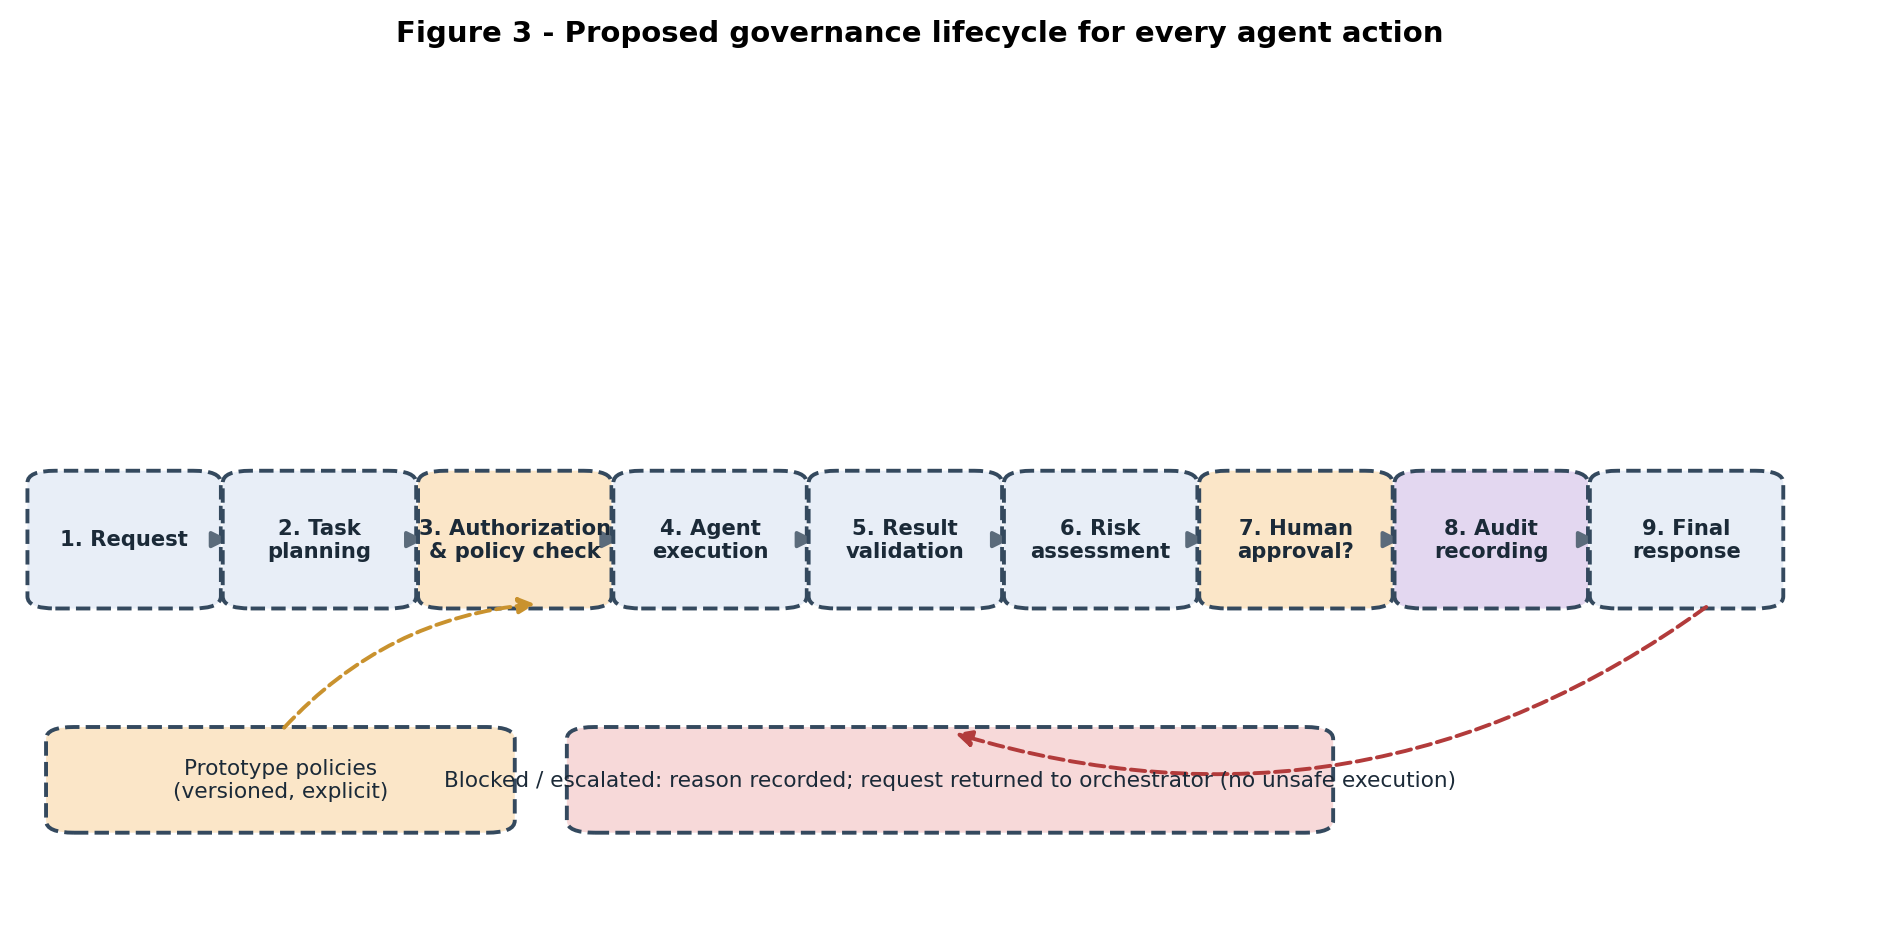
\includegraphics[width=\textwidth]{fig_governance_lifecycle.png}
\caption{Proposed governance lifecycle. Every step after planning is gated; execution cannot occur without an allow decision.}
\label{fig:gov}
\end{figure}

\subsection{Candidate policy rules}
The following explicit rules are proposed for the prototype's policy set. They are \emph{design recommendations}; none is currently enforced in code.
\begin{itemize}
\item \textbf{Read-only analysis} may proceed when the requester is authorized.
\item \textbf{Financial adjustments} require evidence and independent validation.
\item \textbf{High-impact actions} require human approval when policy specifies.
\item \textbf{Missing or contradictory evidence} must trigger escalation, never silent execution.
\item \textbf{Agents must not bypass governance}; consequential actions are fail-closed.
\end{itemize}

\subsection{Security principles}
\paragraph{Least privilege.} Each agent receives only the data and tools its role requires; adapters are read-only.
\paragraph{Input validation.} All messages are schema-validated before dispatch (the implemented analysis package already demonstrates schema validation for source data).
\paragraph{Evidence requirements.} Recommendations carry evidence references; a recommendation without resolvable evidence is rejected.
\paragraph{Controlled tool access.} Tools are exposed through explicit interfaces, not arbitrary execution.
\paragraph{Separation of recommendation and execution.} Agents propose; Governance authorizes; only an authorized executor acts. This mirrors internal-control principles \cite{coso2013,sox2002}.

\subsection{What is enforced versus recommended}
\textbf{Enforced today:} nothing at the agent layer. \textbf{Recommended:} the entire governance lifecycle, the policy rules above, and the audit linkage. The repository does not demonstrate technical enforcement of any of these, and this report does not claim otherwise. The design aligns with recognised AI-governance guidance \cite{nistAirmf2023,nistAi6001,iso42001}.

% ===========================================================================
\section{Dataset and Agent Mapping}
% ===========================================================================
This section maps each agent to the available dataset fields. It does \emph{not} repeat the dataset analysis; the authoritative reference is the project's \emph{Dataset Report} (Deliverable~2). All counts below are measured there and reproduced by the implementation. Table~\ref{tab:map} uses the following categories: \textbf{Direct} (a source field is directly usable), \textbf{Derived} (computed from source fields), and \textbf{Absent} (the dataset cannot supply the item).

\begin{longtable}{L{2.15cm}L{3.0cm}L{2.6cm}L{3.1cm}L{3.1cm}}
\caption{Agent-by-agent mapping of required data, available fields, derived features, supported tasks and unavoidable gaps.}\label{tab:map}\\
\toprule
\textbf{Agent} & \textbf{Required data} & \textbf{Available (source)} & \textbf{Derived features} & \textbf{Unsupported (absent)} \\
\midrule
\endfirsthead
\toprule
\textbf{Agent} & \textbf{Required data} & \textbf{Available (source)} & \textbf{Derived features} & \textbf{Unsupported (absent)} \\
\midrule
\endhead
Orchestrator & Task/state; entity links & \code{order\_id}, \code{customer\_id}, invoice, dates & Task graph over linked records & Agent coordination logs (native) \\
E-Commerce & Orders, items, payments, reviews, stock lines & Olist status/\allowbreak timestamps/\allowbreak payments/\allowbreak reviews; Retail invoice/\allowbreak quantity/\allowbreak price/\allowbreak date/\allowbreak country & Monthly volume, status mix, category revenue, cancellation rate & Live sessions; Retail order status \\
Inventory & Products, quantities, stock & \code{product\_id}, item prices; \code{StockCode}, \code{Quantity} & Units sold, demand variability, velocity ranking & \textbf{Stock-on-hand, replenishment, movements} \\
Accounting & Payments, order value, ledger & Olist \code{payment\_value}/\allowbreak\code{price}/\allowbreak\code{freight}; Retail line value & Order reconciliation proxy; revenue totals & \textbf{General ledger, tax, settlement, chart of accounts} \\
Risk / Anomaly & Amounts, timing, quantity flags & Delivery timestamps, prices, \code{Quantity}, \code{C} prefix & IQR outliers, temporal inconsistencies, negative/\allowbreak zero signals & \textbf{Verified fraud labels} \\
Governance & Policies, permissions & Structured fields usable as rule inputs & Threshold rules (e.g.\ freight ratio) & \textbf{Policies, permissions, approvals} \\
Audit & Event log; evidence keys & Business record keys & Evidence references; input hashes & Native audit log / chain of custody \\
\bottomrule
\end{longtable}

\paragraph{Explicit absences.} The following are \textbf{absent from both datasets} and are therefore prototype responsibilities: inventory snapshots and stock movements; verified fraud labels; general-ledger and tax data; explicit governance-policy records; and native multi-agent execution logs. Related measured caveats from the \emph{Dataset Report}: Online Retail II has 22.77\% missing customer identifiers; Olist geolocation has 26.18\% exact duplicate rows; neither has returns/refunds as a first-class table.

% ===========================================================================
\section{End-to-End Workflow Scenarios}
% ===========================================================================
Four scenarios illustrate coordinated behaviour. \textbf{All four are proposed workflows}; none has been executed. Each figure is a proposed sequence diagram with decision and failure points.

\subsection{Scenario A --- Order and payment reconciliation}
An order-related request is received; relevant order and payment records are retrieved; item totals (price + freight) are compared with payment totals per order; discrepancies beyond a threshold are escalated; governance is applied; a recommendation and audit record are produced. This scenario has the strongest empirical anchor: 99.62\% of the 98{,}665 orders with both items and payments agree within one cent (measured). Failure cases: orders lacking items or payment (775 and 1 respectively) are reported as gaps, not reconciled.

\begin{figure}[H]\centering
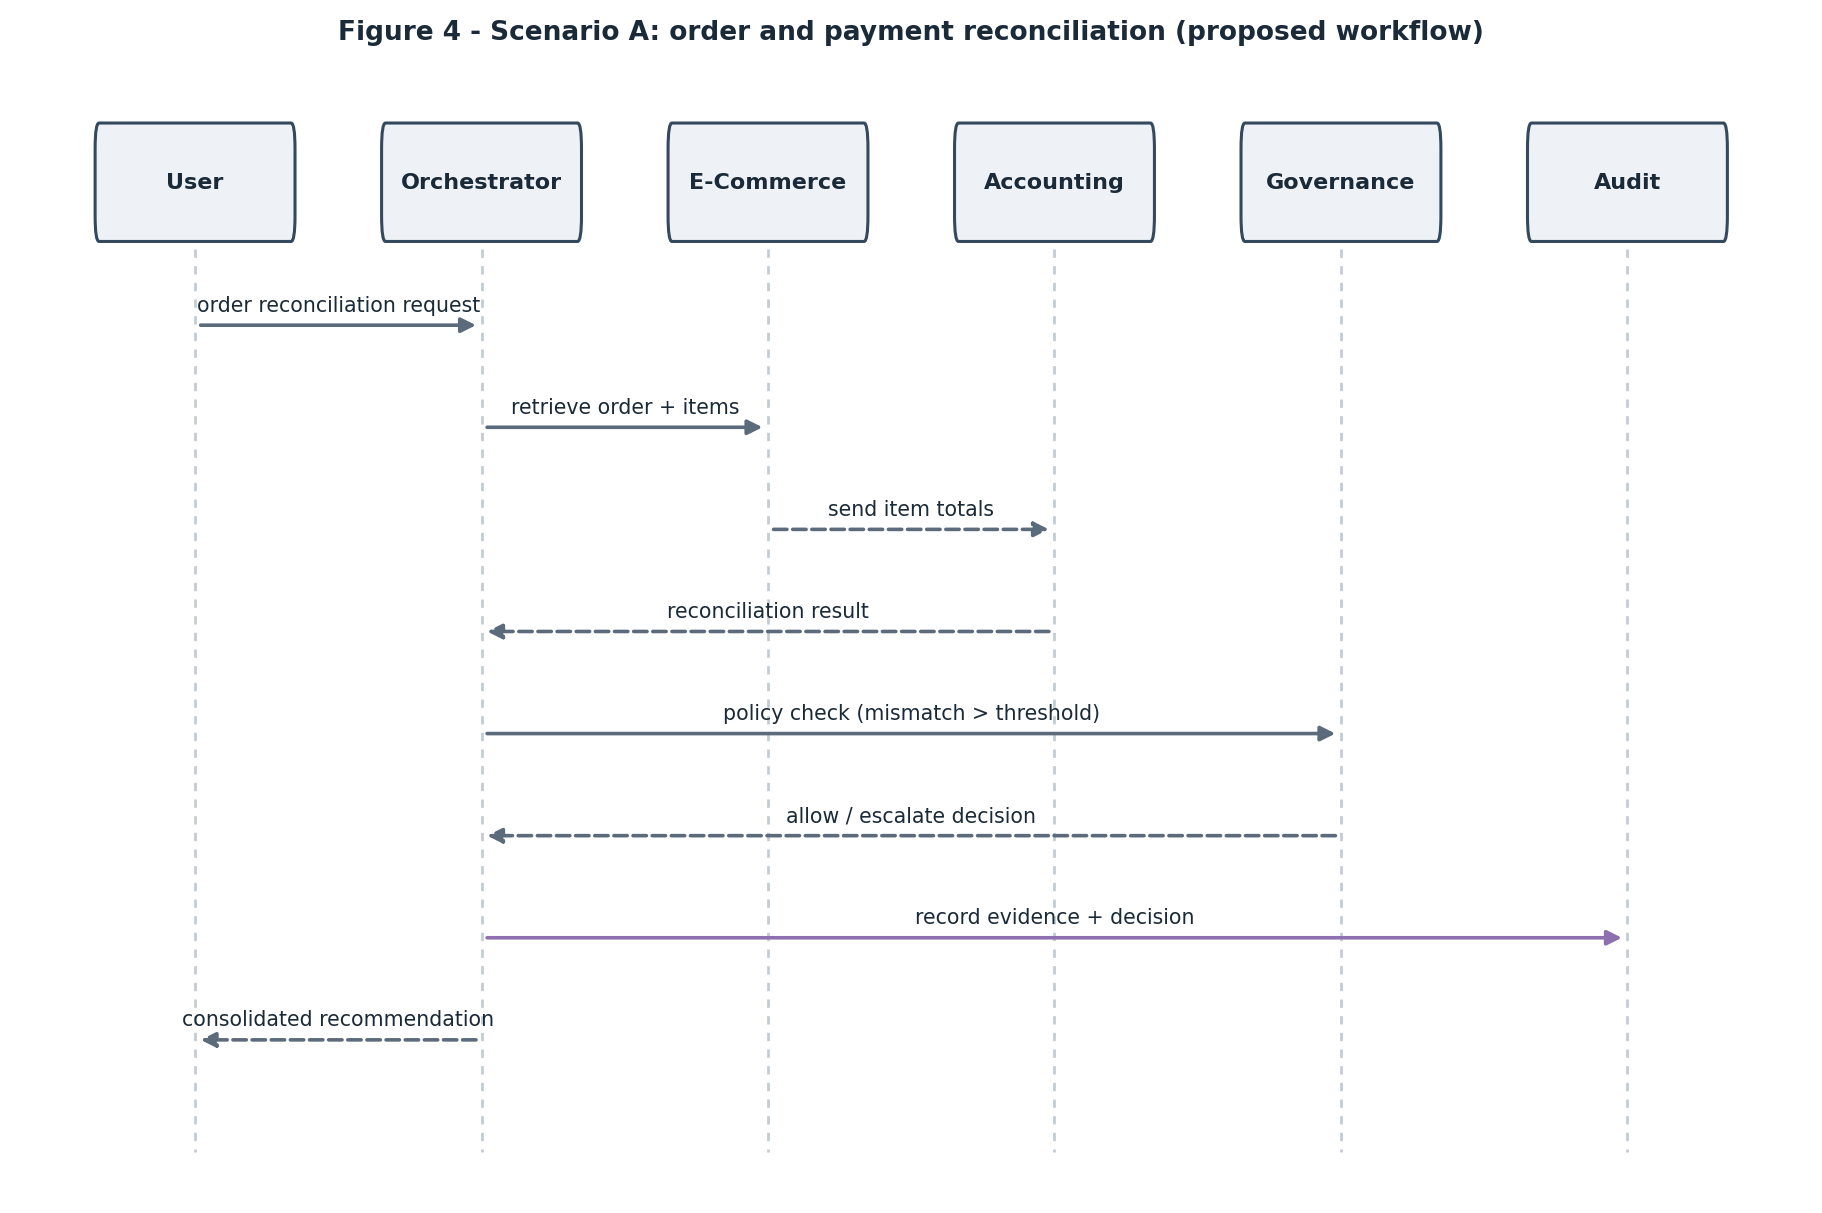
\includegraphics[width=\textwidth]{fig_scenario_a.png}
\caption{Scenario A (proposed): order and payment reconciliation with governance gate and audit record.}
\label{fig:scenA}
\end{figure}

\subsection{Scenario B --- Transaction anomaly investigation}
A transaction is analysed; a candidate anomaly is identified (e.g.\ a negative quantity on a non-cancellation invoice, or a delivered-before-carrier order); supporting evidence is gathered; the Accounting agent checks the relevant financial relationship; risk and governance rules are applied; the case is escalated when evidence is insufficient. This scenario is supported by the measured Online Retail II signals (12{,}326 and 10{,}624 negative-quantity lines per sheet; 8{,}292 cancellation invoices combined) and the 23 Olist delivered-before-carrier orders. Failure cases: the absence of fraud labels means only candidate signals can be produced.

\begin{figure}[H]\centering
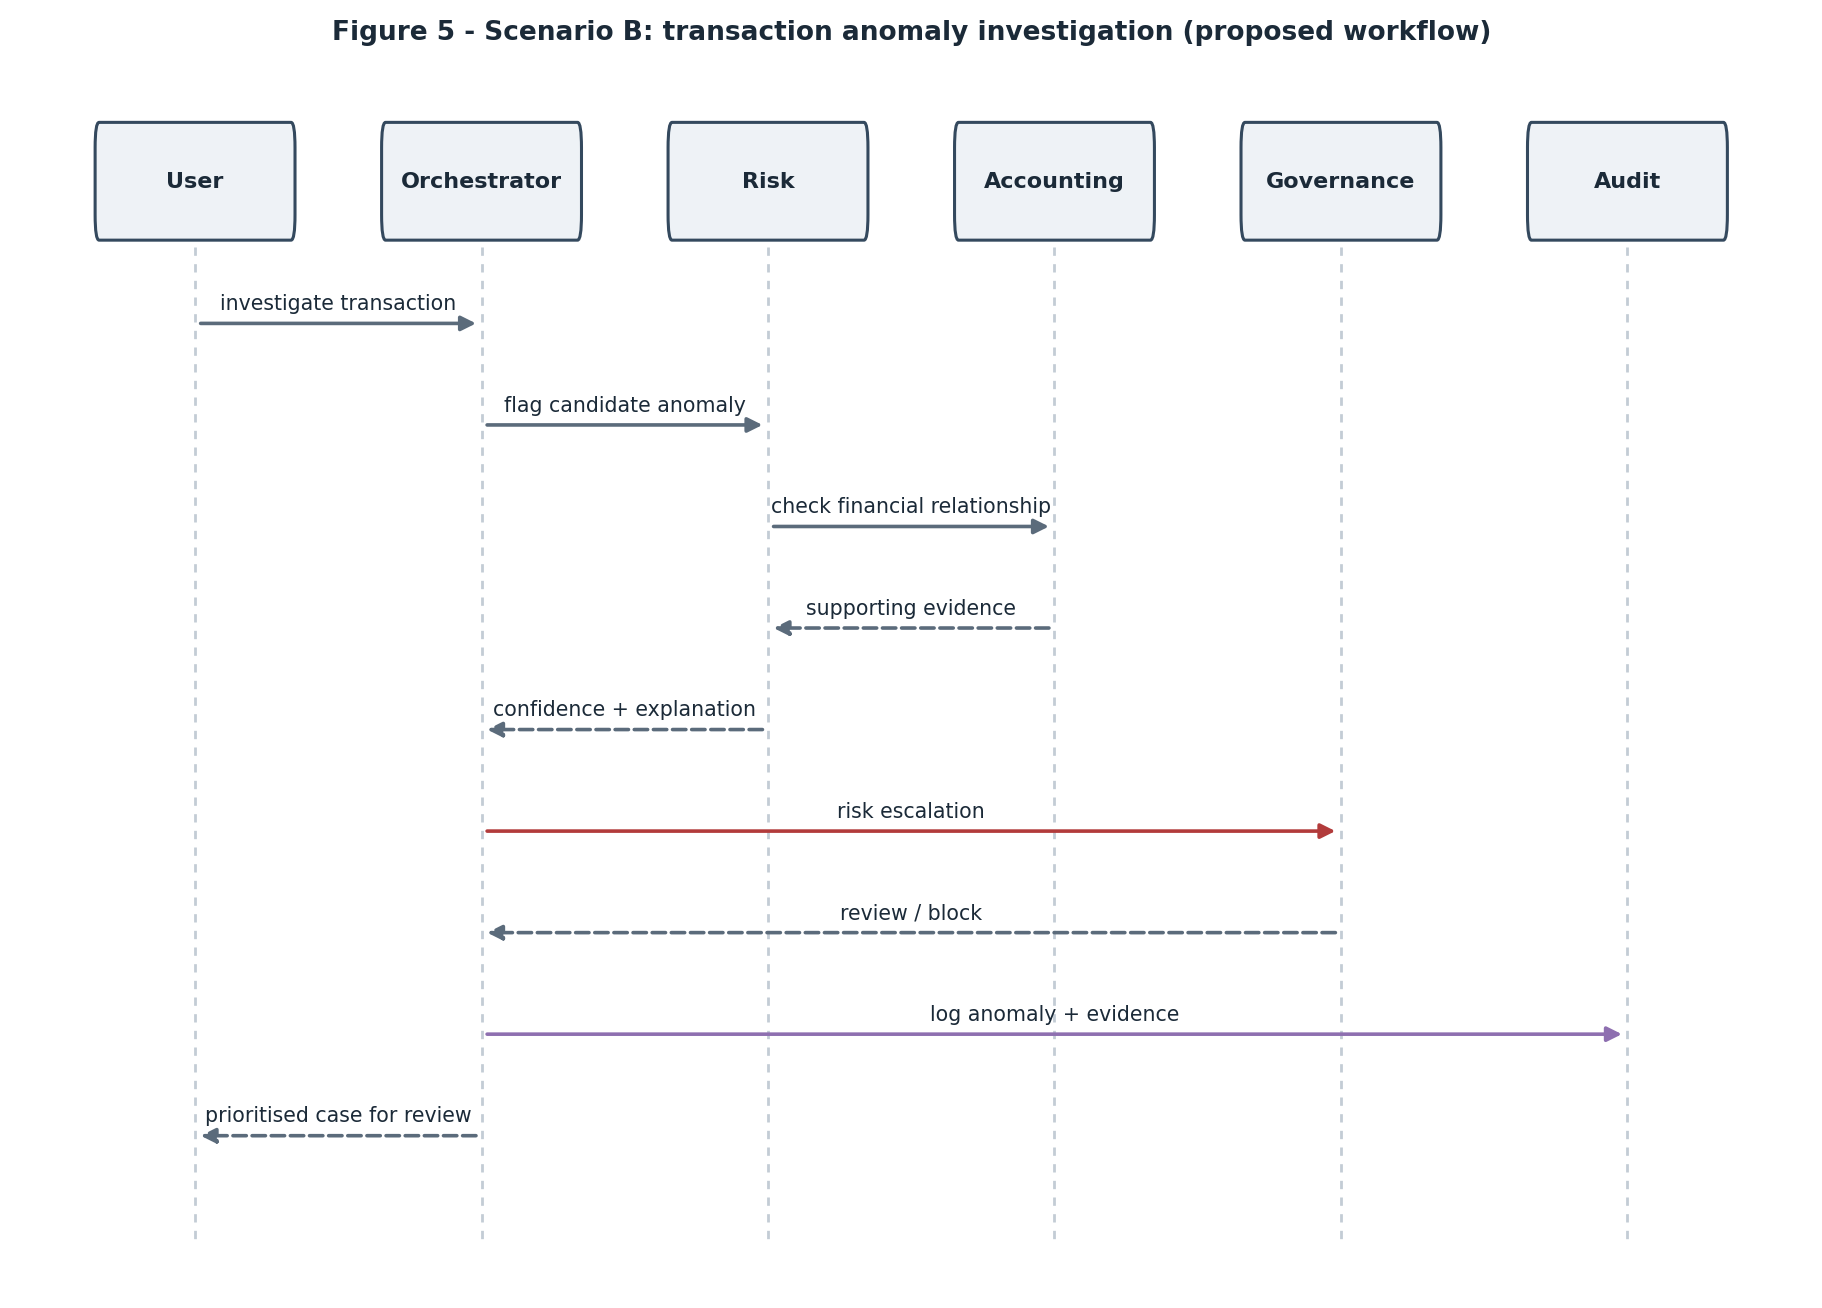
\includegraphics[width=\textwidth]{fig_scenario_b.png}
\caption{Scenario B (proposed): anomaly investigation with accounting cross-check and escalation.}
\label{fig:scenB}
\end{figure}

\subsection{Scenario C --- Inventory risk analysis}
Product and order-item patterns are analysed; demand indicators are estimated where possible; inventory-related information gaps are identified; a \emph{qualified} recommendation is produced; and the workflow explains why actual stock decisions require additional inventory data. This scenario is deliberately limited: neither dataset contains stock-on-hand. Failure cases: missing product metadata (610 Olist products) reduces coverage.

\begin{figure}[H]\centering
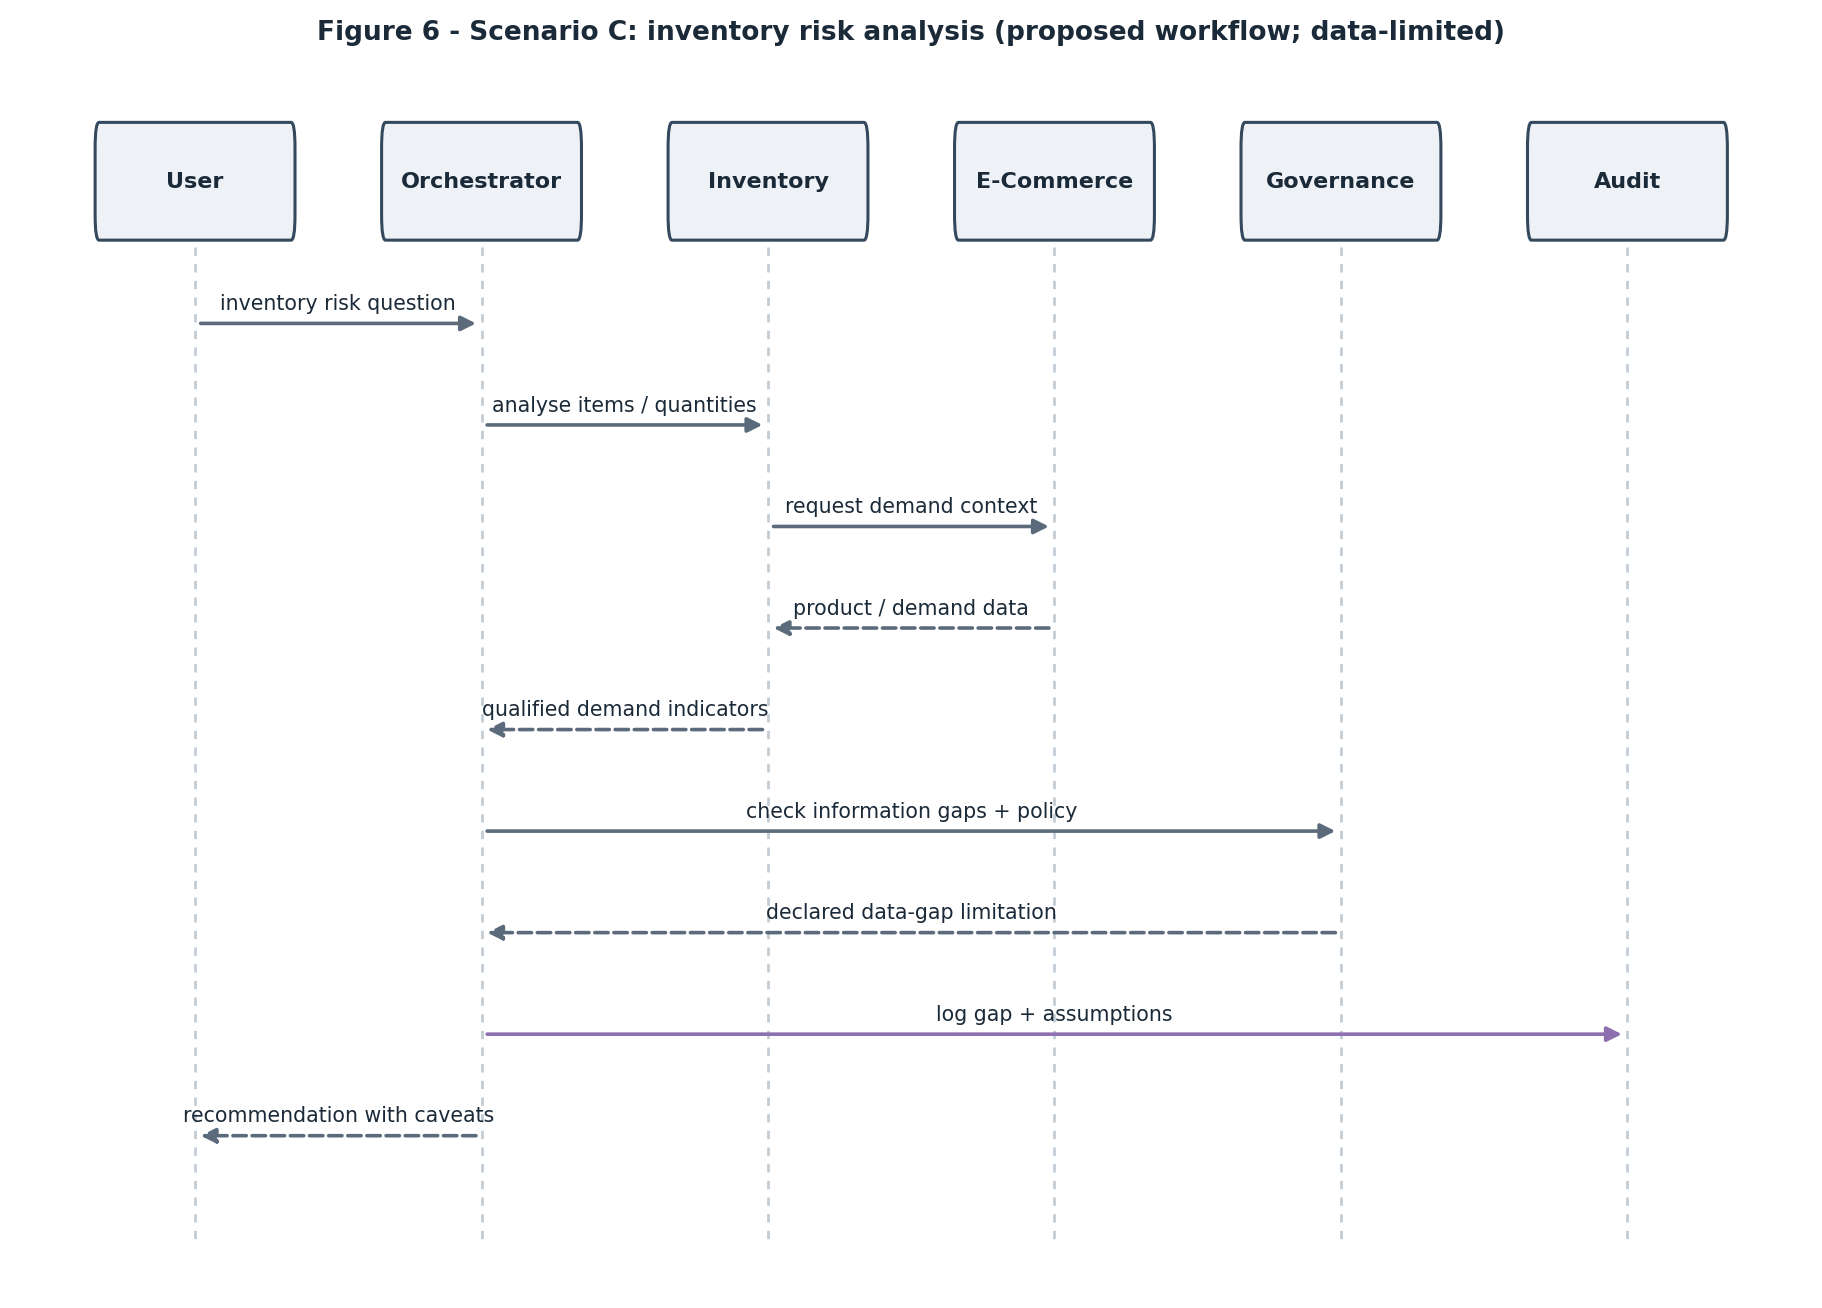
\includegraphics[width=\textwidth]{fig_scenario_c.png}
\caption{Scenario C (proposed): inventory risk analysis with explicit data-gap declaration.}
\label{fig:scenC}
\end{figure}

\subsection{Scenario D --- Governance rejection}
An agent proposes a restricted or insufficiently supported action; the Governance agent checks the policy; the action is rejected or escalated; the decision and reason are recorded for audit. This scenario exercises the fail-closed behaviour that the architecture requires. Failure cases: if the policy set is missing or contradictory, the action must be escalated, never executed.

\begin{figure}[H]\centering
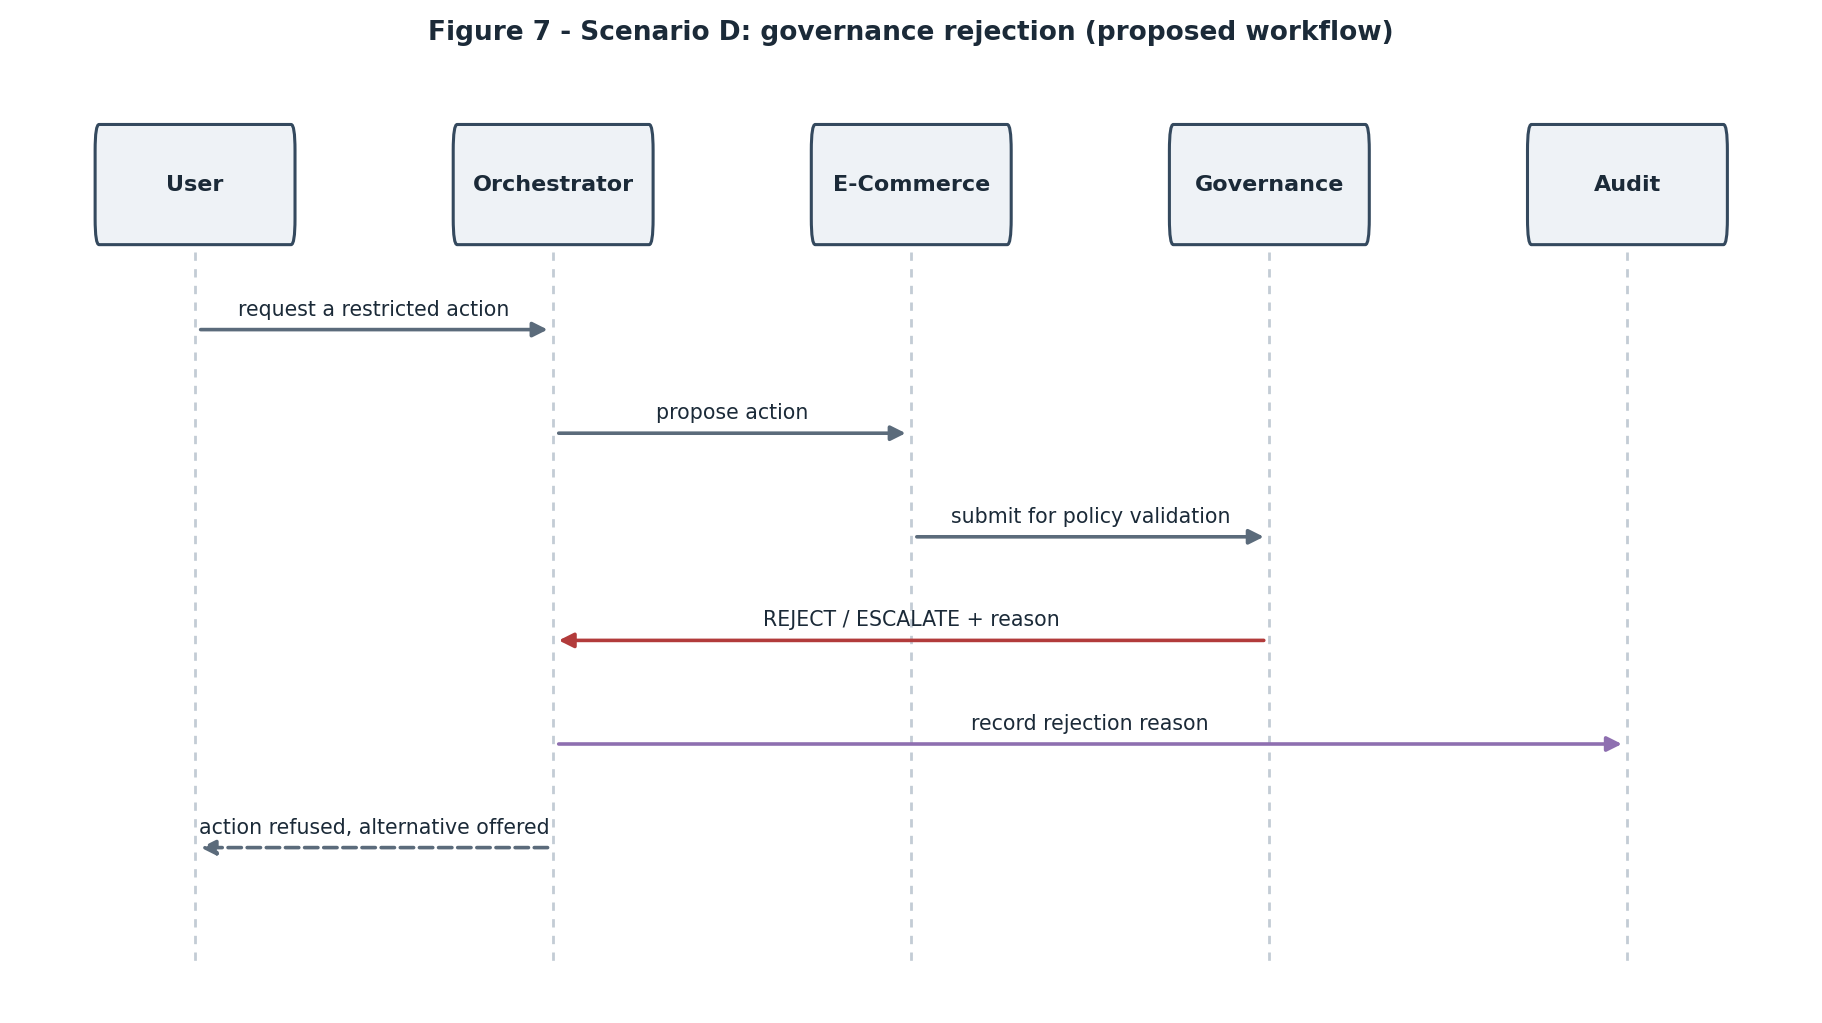
\includegraphics[width=\textwidth]{fig_scenario_d.png}
\caption{Scenario D (proposed): governance rejection with recorded reason and audit entry.}
\label{fig:scenD}
\end{figure}

% ===========================================================================
\section{Data Contracts and Audit Schema}
\label{sec:contracts}
The repository contains \textbf{no implemented message, task, anomaly, policy or audit schemas}; what follows are \emph{proposed} contracts. The only implemented ``schemas'' are the source-data column expectations in the analysis package (\code{olist.EXPECTED\_COLUMNS}, \code{online\_retail.EXPECTED\_COLS}), which are not agent contracts. JSON examples are illustrative and clearly labelled as proposed.

\paragraph{Task request (proposed).}
\begin{verbatim}
{ "task_id": "t-0001", "correlation_id": "req-7f3a",
  "target_agent": "accounting", "task_type": "reconcile_order",
  "scope": {"dataset": "olist", "order_id": "..."},
  "deadline": "2026-01-01T00:00:00Z" }
\end{verbatim}

\paragraph{Agent result (proposed).}
\begin{verbatim}
{ "task_id": "t-0001", "status": "success",
  "summary": {"matched": true, "abs_diff": 0.0},
  "evidence_refs": [{"table":"order_payments","key":"..."},
                    {"table":"order_items","key":"..."}],
  "agent": "accounting", "timestamp": "..." }
\end{verbatim}

\paragraph{Anomaly finding (proposed).}
\begin{verbatim}
{ "anomaly_id": "a-0012", "category": "statistical_outlier",
  "rule": "iqr_quantity", "score": 0.93,
  "explanation": "quantity beyond IQR fence",
  "evidence_refs": [{"table":"online_retail_II","key":"..."}],
  "label": "candidate_anomaly" }
\end{verbatim}

\paragraph{Policy decision (proposed).}
\begin{verbatim}
{ "decision_id": "p-0044", "action": "post_adjustment",
  "policy_id": "FIN-002", "decision": "escalate",
  "reason": "requires human approval",
  "human_approval_required": true }
\end{verbatim}

\paragraph{Audit event (proposed).} Table~\ref{tab:audit} lists the proposed audit-event fields. These events are prototype-generated; they are \emph{not} attributes of either dataset. The schema deliberately excludes personal data.

\begin{table}[H]
\centering
\small
\caption{Proposed audit event schema (prototype-generated; not implemented).}
\label{tab:audit}
\begin{tabular}{L{3.4cm}L{3.6cm}L{7.0cm}}
\toprule
\textbf{Field} & \textbf{Type} & \textbf{Meaning} \\
\midrule
\code{event\_id} & string (UUID) & Unique identifier of the audit event \\
\code{timestamp} & datetime & When the action occurred \\
\code{agent} & string & Agent that acted \\
\code{action} & string & Operation performed \\
\code{policy\_id} & string & Experimental governance rule evaluated \\
\code{policy\_decision} & enum & allow / block / escalate \\
\code{evidence\_refs} & list & Source records (table + key) used as evidence \\
\code{input\_digest} & string (hash) & Hash of the input records (precedent: \code{config.sha256\_file}) \\
\code{outcome} & enum & success / failure / pending \\
\code{notes} & string & Free-text rationale (no personal data) \\
\bottomrule
\end{tabular}
\end{table}

% ===========================================================================
\section{Evaluation Methodology}
% ===========================================================================
\textbf{No agent experiments have been run}, so this section is a \emph{proposed} evaluation plan; no results are reported. The plan follows a design-science structure of build-and-evaluate \cite{hevner2004}.

\paragraph{Metrics.} Table~\ref{tab:metrics} classifies metrics by whether they can be computed immediately from data, or require the prototype, annotations, or external ground truth.

\begin{table}[H]
\centering
\small
\caption{Proposed evaluation metrics and their data requirements.}
\label{tab:metrics}
\begin{tabular}{L{5.0cm}L{3.4cm}L{5.6cm}}
\toprule
\textbf{Metric} & \textbf{Status} & \textbf{Basis / requirement} \\
\midrule
Data validation error rate & Immediate & Schema/key/integrity checks (implemented) \\
Reconciliation mismatch rate & Immediate (proxy) & Olist item-vs-payment (99.62\% within one cent measured) \\
Record duplication rate & Immediate & Exact-duplicate counts (implemented) \\
Anomaly flag rate & Immediate (rules) & Rule-based flags on quantities/prices/timestamps \\
Anomaly precision / recall & Requires labels & Needs trustworthy ground-truth annotations (absent) \\
Policy violation detection rate & Requires prototype & Depends on experimental policy definitions \\
False-block rate & Requires prototype & Requires prototype outcomes \\
Task completion rate & Requires prototype & Workflows executed by the Orchestrator \\
Agent coordination failures & Requires prototype & From orchestration traces \\
Audit event completeness & Requires prototype & Coverage over generated audit logs \\
Evidence traceability & Requires prototype & Fraction of decisions with resolvable evidence \\
Latency and computational cost & Requires prototype & Time/cost per agent run \\
\bottomrule
\end{tabular}
\end{table}

\paragraph{Experimental procedure.} For each scenario, run the workflow under (i) a no-agent scripting baseline, (ii) a single-agent baseline, and (iii) the full governed multi-agent configuration; compare on the metrics above. Baselines isolate the contribution of coordination and governance from the underlying analytics. Fix random seeds for any stochastic method and version-pin dependencies.

\paragraph{Reproducibility.} Immutable raw inputs with recorded SHA-256 hashes (already produced by the analysis package), machine-readable outputs for every reported number, and a committed script that regenerates results.

\paragraph{Limitations.} Precision/recall for anomalies is not computable without labels; governance metrics depend on policies the prototype itself defines; and single-source, single-period data limit generalisability.

% ===========================================================================
\section{Failure Modes and Limitations}
\label{sec:limitations}
\begin{itemize}
\item \textbf{Incorrect or incomplete source records.} e.g.\ Olist orders without items/\allowbreak payment/\allowbreak review; Retail lines without a customer identifier.
\item \textbf{Missing fields and inconsistent identifiers.} Structural missingness (undelivered timestamps; 22.77\% missing customer IDs), and mixed-type codes in Online Retail II.
\item \textbf{Unsupported inferences.} The design forbids inventing stock levels, ledger balances or fraud labels; any such inference is a failure.
\item \textbf{False positives in anomaly detection.} Candidate signals include legitimate returns/\allowbreak adjustments; without labels these cannot be separated by measurement alone.
\item \textbf{Agent disagreement.} Resolved by escalation, never by silent override.
\item \textbf{Invalid or malformed messages.} Prevented by schema validation; rejected messages fail closed.
\item \textbf{Tool failures and timeouts.} Handled by bounded retries and graceful degradation.
\item \textbf{Governance bypass risks.} Mitigated by making Governance a mandatory chokepoint; until implemented, this risk is open.
\item \textbf{Incomplete audit trails.} Would invalidate traceability claims; the workflow must fail closed if auditing is unavailable.
\item \textbf{Dataset bias and generalisability.} Both datasets cover specific retailers, regions and periods.
\item \textbf{Offline-versus-live gap.} Historical replay cannot evidence autonomous live coordination.
\end{itemize}

\paragraph{Ethical considerations and privacy.} Both datasets are anonymised/pseudonymised public releases but describe real commercial behaviour. The design therefore never reproduces personal identifiers, treats free-text reviews as potentially sensitive, and requires the audit schema to exclude personal data. Any deployment must respect data-protection obligations such as the GDPR \cite{gdpr2016} and the datasets' licences (Online Retail II: CC BY 4.0; Olist: CC BY-NC-SA 4.0).

% ===========================================================================
\section{Implementation Roadmap}
% ===========================================================================
The roadmap is ordered by dependency and adapted to actual progress. Only milestone~1 is substantially complete.
\begin{enumerate}
\item \textbf{Data interfaces and validation.} \emph{Partially implemented.} The analysis package provides read-only loading, schema validation, key/integrity checks and profiling; a prototype of the ingestion/validation layer exists. Remaining: expose these as stable agent-facing interfaces and canonical events.
\item \textbf{Agent contracts and coordination.} \emph{Proposed.} Define message/task schemas and an Orchestrator that executes a task graph.
\item \textbf{Specialised analytical capabilities.} \emph{Proposed.} Wrap the existing computations into the E-Commerce, Inventory, Accounting and Risk agents.
\item \textbf{Governance enforcement.} \emph{Proposed.} Implement the policy set and the allow/block/escalate chokepoint.
\item \textbf{Audit and traceability.} \emph{Proposed.} Implement the append-only audit store and evidence linkage.
\item \textbf{Integration and end-to-end testing.} \emph{Proposed.} Execute the four scenarios across both adapters.
\item \textbf{Evaluation and reproducibility.} \emph{Proposed.} Run the evaluation protocol with baselines.
\item \textbf{Documentation and deployment readiness.} \emph{Proposed.} Package, document and harden.
\end{enumerate}

% ===========================================================================
\section{Conclusion and Future Work}
% ===========================================================================
This report specifies a governance-first, seven-agent architecture for autonomous e-commerce and accounting operations and documents its status honestly. The principal finding is a clear gap between design and implementation: \textbf{no agent is implemented}. The project currently contains a solid, tested data-analysis and validation layer and a dataset inspector, on which the agents can be built, but it contains no orchestration, messaging, policy, or audit code. The contribution of this report is therefore a concrete, evidence-grounded specification and roadmap, not a description of a working multi-agent system.

Future work is the roadmap itself: promote the analysis package into stable agent-facing interfaces, implement the Orchestrator and specialist agents, implement and test the governance chokepoint and the audit ledger, execute the four scenarios, and evaluate against the proposed baselines. Only after those steps could the project legitimately claim a functioning governed multi-agent system, and only with a labelled dataset could it claim anomaly-detection accuracy.

% ===========================================================================
% REFERENCES
% ===========================================================================
\bibliographystyle{plain}
\bibliography{references}

% ===========================================================================
% APPENDIX
% ===========================================================================
\appendix
\section{Repository Inventory and Reproduction}
\label{app:inventory}
\subsection*{A.1 What the repository actually contains}
\begin{itemize}
\item \code{README.md} --- empty.
\item \code{src/} --- empty (no source code).
\item \code{datasets/olist/} --- nine Olist CSV files (read-only).
\item \code{datasets/online\_retail\_ii/online\_retail\_II.xlsx} --- two worksheets (read-only).
\item \code{reports/dataset\_report/} --- the \emph{Dataset Report}: \code{dataset\_report.tex/.pdf}, \code{references.bib}, and the implemented analysis package \code{analysis/} with \code{analysis\_results/}, \code{figures/} and \code{tests/}.
\item \code{reports/dataset\_selection\_table/} --- the project/dataset overview: \code{main.tex/.pdf}, \code{scripts/inspect\_datasets.py}, and CSV/JSON artifacts.
\end{itemize}

\subsection*{A.2 Implemented analysis package (evidence)}
\code{reports/dataset\_report/analysis/} exposes: \code{config} (paths, \code{sha256\_file}, writers); \code{profiling} (\code{column\_profile}, \code{exact\_duplicates}, \code{numeric\_stats}, \code{categorical\_stats}, \code{temporal\_profile}, \code{key\_check}, \code{value\_counts\_table}); \code{olist} (\code{load\_tables}, \code{validate\_schema}, \code{referential\_integrity}, \code{\_join\_expansion}, \code{run}); \code{online\_retail} (\code{load\_sheets}, \code{\_clean}, \code{\_clean\_code}, \code{\_strip\_nullable}, \code{\_invoice\_kind}, \code{\_sheet\_quality}, \code{run}); \code{figures}; \code{compare} (\code{dataset\_inventory}, \code{dataset\_comparison}, \code{agent\_suitability}). Entry point: \code{python -m analysis}.

\subsection*{A.3 Toolchain observed}
Python 3.10.11; pandas 2.3.3; NumPy 1.26.4; matplotlib 3.10.7; seaborn 0.13.2; openpyxl 3.1.5; pytest 9.1.0. The dataset-selection inspector uses only the Python standard library. LaTeX (MiKTeX) with \code{pdflatex}/\code{bibtex} compiles this report.

\subsection*{A.4 Tests executed}
The dataset-analysis tests (\code{reports/dataset\_report/tests/test\_analysis.py}) were run with \code{python -m pytest tests -q}; \textbf{13 tests passed}. These tests validate data-metric definitions (missing-value preservation, duplicate counting, key checks, referential integrity, sign counts, temporal profiling, cancellation detection, revenue definitions, schema validation). \textbf{No agent-level tests exist.}

\subsection*{A.5 Reproducing this report's diagrams}
From \code{reports/Agents reports/figures}: run \code{python make\_figures.py} to regenerate all diagrams as PNGs. The diagrams are schematic and are not measured data.

\end{document}
